\label{sec:impacts_inclusive}
\providecommand{\impactswidthscale}{0.6}
%% The \nonprompt photon contribution is estimated using the data-driven approach.
%% The variable considered is $m_{\PZ\PZ\PGg}$.
%% The impacts of the systematic uncertainties on the expected results is shown in Figure \ref{fig:inclusive_cutID_phoCR_mZZGloose}.

\begin{figure}
  \centering
  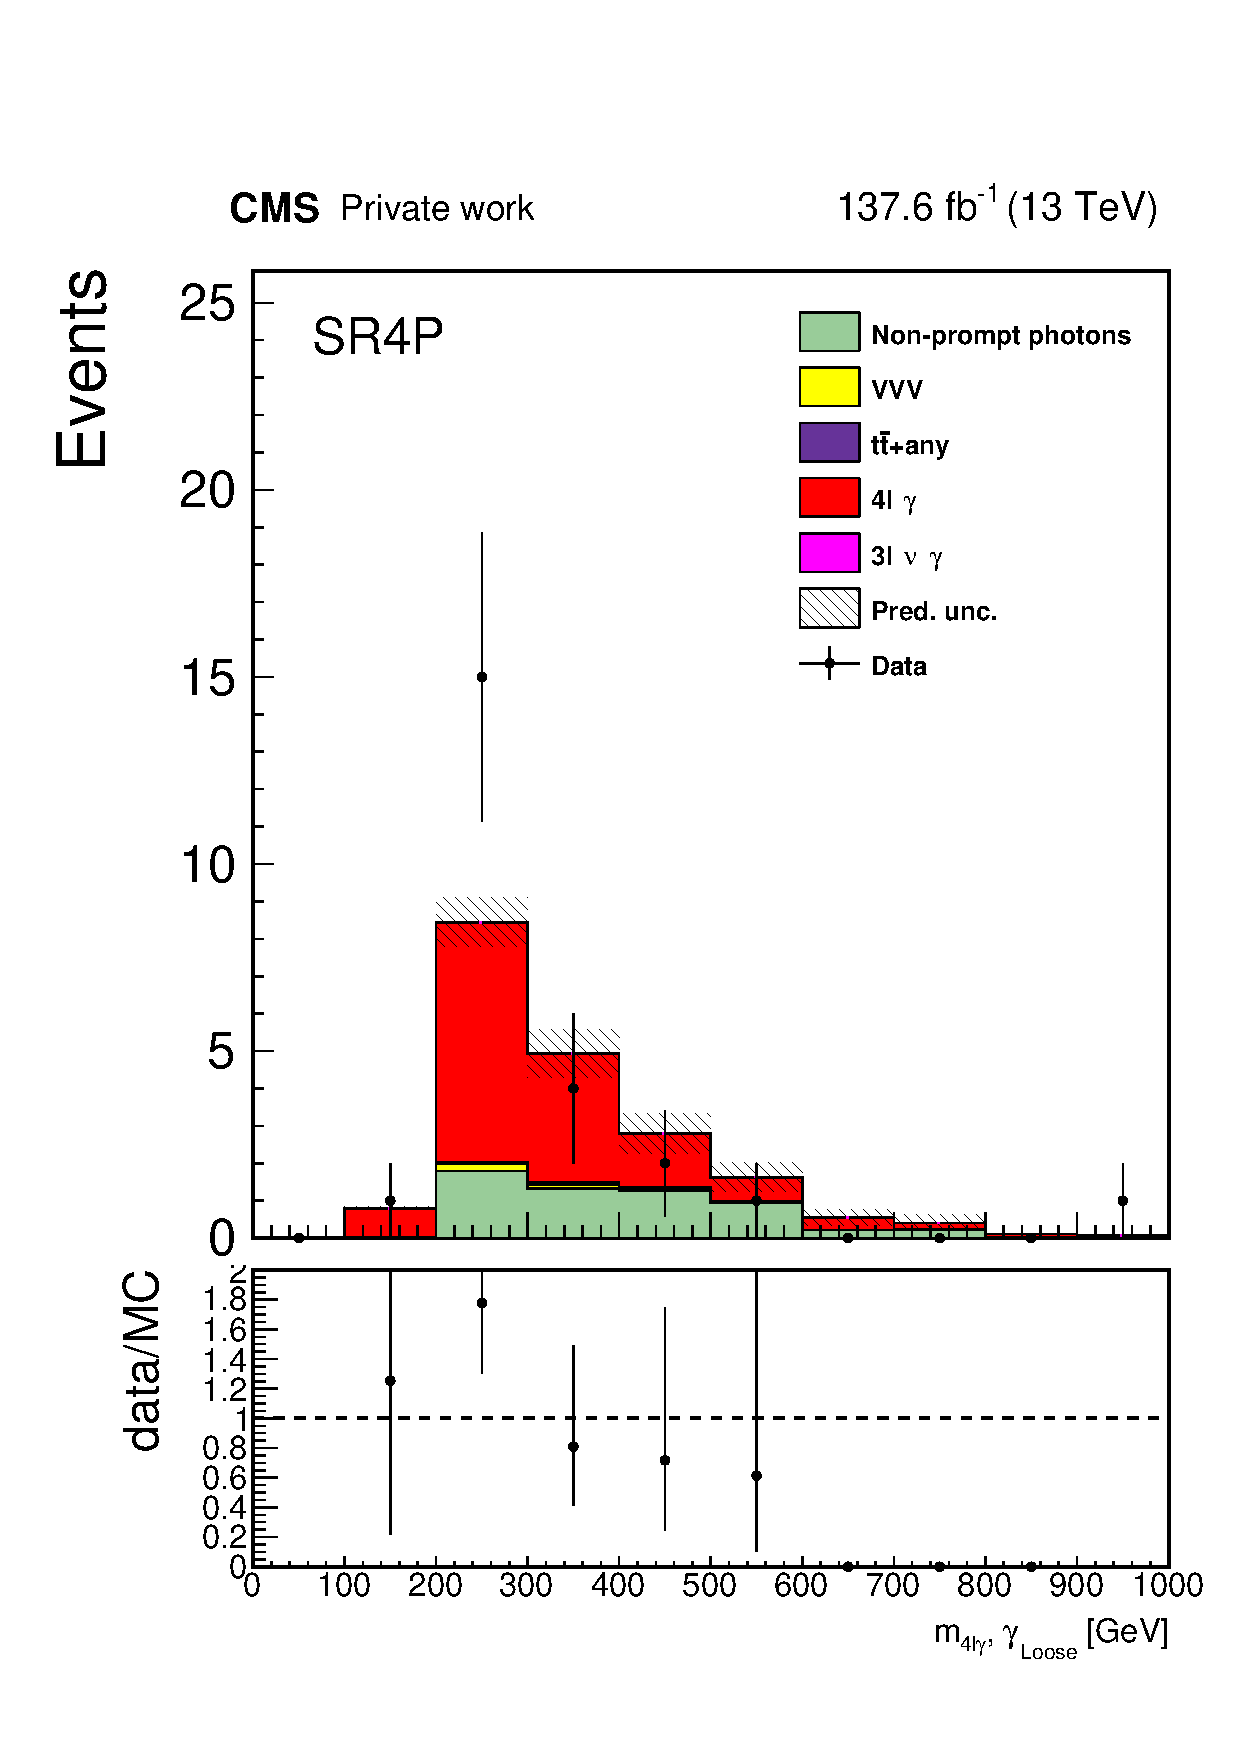
\includegraphics[height=0.33\textheight]{Figures/dataMC/Run2/phoCR/SR4P/SYS_mZZGloose_central_pow.pdf}
  \hfill
  \includegraphics[height=0.33\textheight]{Figures/combine/noPixVeto/Run2_SR4P_phoCR_lepCR_mZZGloose_impacts.pdf}
  \caption{Distribution and impacts of the systematic uncertainties on the signal strength fit
    on the mass of the $\PZ\PZ\PGg$ system,
    using the Loose working point of the photon cut-based ID.
    The data-driven estimate for \nonprompt photons is used.
    The FSR cut is not applied.
  }
  \label{fig:inclusive_cutID_phoCR_mZZGloose}
\end{figure}

\begin{figure}
  \centering
  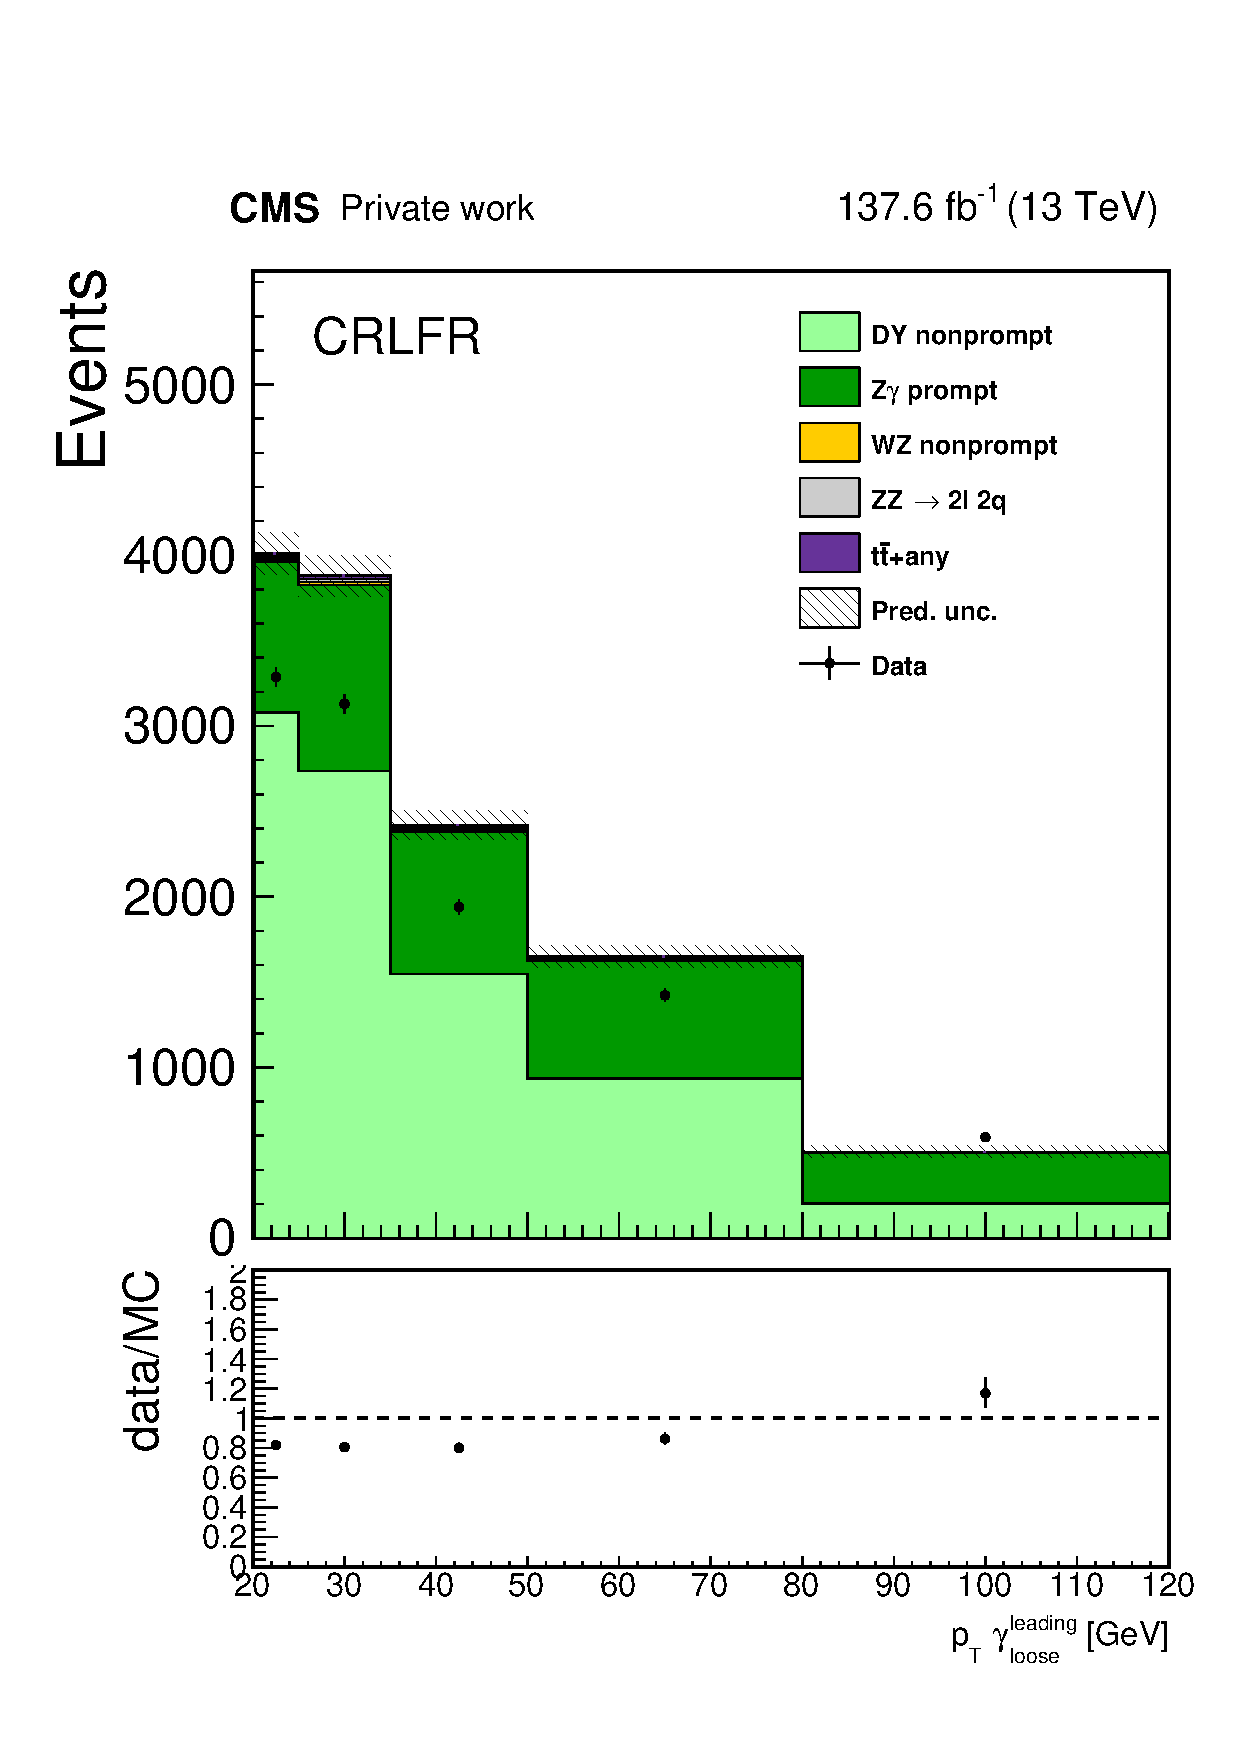
\includegraphics[height=0.33\textheight]{Figures/dataMC/Run2/lepCR/SR4P/lead_loose_pt_pow.pdf}
  \hfill
  \includegraphics[height=0.33\textheight]{Figures/combine/noPixVeto/Run2_SR4P_phoMC_lepCR_loosept_impacts.pdf}
  \caption{Distribution and impacts of the systematic uncertainties on the signal strength fit
    on the transverse momentum of the photon,
    using the Loose working point of the photon cut-based ID.
    \Nonprompt photons are estimated from simulation.
    The FSR cut is not applied.
  }
  \label{fig:inclusive_cutID_phoMC_loosept}
\end{figure}

\begin{figure}
  \centering
  \includegraphics[height=0.33\textheight]{Figures/dataMC/Run2/lepCR/SR4P/SYS_wp90pt_central_pow.pdf}
  \hfill
  \includegraphics[height=0.33\textheight]{Figures/combine/noPixVeto/Run2_SR4P_phoMC_lepCR_mZZGwp90_impacts.pdf}
  \caption{Distribution and impacts of the systematic uncertainties on the signal strength fit
    on the mass of the $\PZ\PZ\PGg$ system,
    using the \texttt{wp90} working point of the photon MVA ID.
    \Nonprompt photons are estimated from simulation.
    The FSR cut is not applied.
  }
  \label{fig:inclusive_mvaID_phoMC_mZZGwp90}
\end{figure}

\begin{figure}
  \centering
  \includegraphics[height=0.33\textheight]{Figures/dataMC/Run2/lepCR/SR4P/SYS_wp80pt_central_pow.pdf}
  \hfill
  \includegraphics[height=0.33\textheight]{Figures/combine/noPixVeto/Run2_SR4P_phoMC_lepCR_mZZGwp80_impacts.pdf}
  \caption{Distribution and impacts of the systematic uncertainties on the signal strength fit
    on the mass of the $\PZ\PZ\PGg$ system,
    using the \texttt{wp80} working point of the photon MVA ID.
    \Nonprompt photons are estimated from simulation.
    The FSR cut is not applied.
  }
  \label{fig:inclusive_mvaID_phoMC_mZZGwp80}
\end{figure}

\begin{figure}
  \centering
  \includegraphics[height=0.33\textheight]{Figures/dataMC/Run2/lepCR/SR4P/SYS_MVAcut_central_pow.pdf}
  \hfill
  \includegraphics[height=0.33\textheight]{Figures/combine/noPixVeto/Run2_SR4P_phoMC_lepCR_MVAcut_impacts.pdf}
  \caption{Distribution and impacts of the systematic uncertainties on the signal strength fit
    on the yield in the various bins of the photon MVA ID.
    \Nonprompt photons are estimated from simulation.
    The FSR cut is not applied.
  }
  \label{fig:inclusive_kin_phoMC_MVAcut}
\end{figure}
